\documentclass{article}
\usepackage{graphicx}
\usepackage[colorlinks=true, urlcolor=blue]{hyperref}
\usepackage{amsmath}

\title{Homework 2: Game of Life Parallelized}
\author{Zachary Heras}

\begin{document}
	\maketitle
	
	\section{Problem Statement}
	The goal of this assignment is to develop a parallel program that simulates John Conway's \textit{Game of Life}, as part of the parallel and concurrent programming course at Rowan University. The program must accept a single input specifying the grid size, \(N\) (where the grid is \(N\) by \(N\)), another input for the maximum number of iterations the game is allowed to run, and an input for the number of threads that the program is allowed to use. The program's execution time will be evaluated based on a set of test cases provided by the course instructor, Dr. Guo. The program is to be written in C using the OpenMP library and executed on Rowan University's cluster computer. All files associated with this project can be found on \href{https://github.com/ZacharyHeras/parallel_and_concurrent_programming/tree/main/hw2}{GitHub}.

	\section{Program Design}
	This program is based off of the serial version of the program from homework 1. With that in mind, we will only review how the program was parallelized, instead of focusing on the design of the game.
	
	To parallelize the program, parallelization is applied to some functions to improve performance using OpenMP. In the init\_board function, the initialization of non-ghost cells is parallelized using the \texttt{\#pragma omp parallel for} directive, distributing the work across multiple threads. In the main function, the game loop runs inside a parallel region with \texttt{\#pragma omp parallel}. The update\_board function is parallelized by applying \texttt{\#pragma omp for} to the loops that update the game board and by protecting the updated variable with a \texttt{\#pragma omp critical} section to prevent race conditions. The update\_ghost\_cells function is parallelized by dividing the tasks into independent sections with \texttt{\#pragma omp sections}, where each section handles different parts of the ghost cell update (corners, leftmost, rightmost, topmost, and bottommost rows/columns). Notice that the \texttt{parallel} keyword is dropped from the update\_ghost\_cells and update\_board functions’ \texttt{\#pragma omp} clauses. This is done to ensure that the same threads are being used in each game loop, as the parallel region is defined in the main loop. Synchronization is ensured by using \texttt{\#pragma omp single} for tasks like incrementing the iteration counter and printing the board, ensuring these operations are performed by only one thread. In an earlier iteration of the code, I mistakenly used \texttt{\#pragma omp critical} instead of \texttt{\#pragma omp single}. This caused the game board to print multiple times and caused the iterations to increment multiple times during a single iteration. Overall, the second version leverages OpenMP constructs like parallel loops, sections, and critical sections to speed up the game. This will likely lead to faster execution times on multi-core systems like Rowan University’s cluster computer.
	
	To compile the program, use the command \texttt{gcc -fopenmp -o hw2 -DSET\_SEED hw2.c}, or use the command \texttt{gcc -fopenmp -o hw2 -DSET\_SEED -DDEBUG\_PRINT hw2.c} to print out the game board after each iteration. To run the program, use the command \texttt{./hw2 N I T}, where \texttt{N} is the game board side size, \texttt{I} is the number of iterations, and \texttt{T} is the thread count.
	
	To verify that the program was functioning correctly, the program was run with 1 thread and compared to the output of the program with 2 or more threads specified.

	\section{Test Cases}
	Once the program was made, the next step was to run tests to examine the execution time for each predetermined test. The tests that will be run are shown in table \ref{table1} below.

	\section{Test System Configuration}
	Each test was executed on the Rowan cluster computer, utilizing one of the \texttt{csm-com-[001-012]} nodes. A Slurm script was written for each test to preserve the test setup information. The scripts were stored in \texttt{.sh} files, following the naming pattern \texttt{run\_hw2\_x\_y.sh}, where \texttt{x} represents the test case. For this test suite, a board size of 5000, and a max iterations of 5000 were used.

	\section{Analysis and Conclusions}
	Below, figure \ref{figure1}, figure \ref{figure2} and table \ref{table1} describe the resulting execution times and other metrics.
	
	The speedup (\(s\)) is defined as the ratio of the serial execution time (\(t_{\text{serial}}\)) to the parallel execution time (\(t_{\text{parallel}}\)):

\[s = \frac{t_{\text{serial}}}{t_{\text{parallel}}}\]

The efficiency (\(\eta\)) is the ratio of Speedup to the number of processors (\(P\)):

\[\eta = \frac{s}{p}\]

From both the table and the figures, we see a decrease in execution time as the thread count increases up until 8 threads. After 8 threads the execution time begins to decrease. This was unexpected, and is likely because of a more complicated cache miss issue. This unexpected outcome affected the results of the speedup and efficiency as well. The speed up began to sharply decrease after 8 threads was exceeded, and efficiency got significantly worse after 8 threads as a result. One thread can be thought of as sequential, and as seen it is slower in execution time than all of the larger thread count execution times.
	
	\begin{figure}
		\centering
		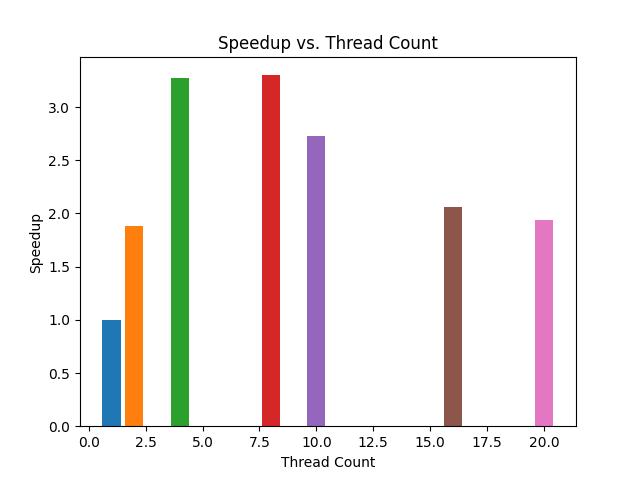
\includegraphics[width=0.8\textwidth]{Figure_1}
		\caption{Speedup vs. thread count.}
		\label{figure1}
	\end{figure}
	
	\begin{figure}[ht]
		\centering
		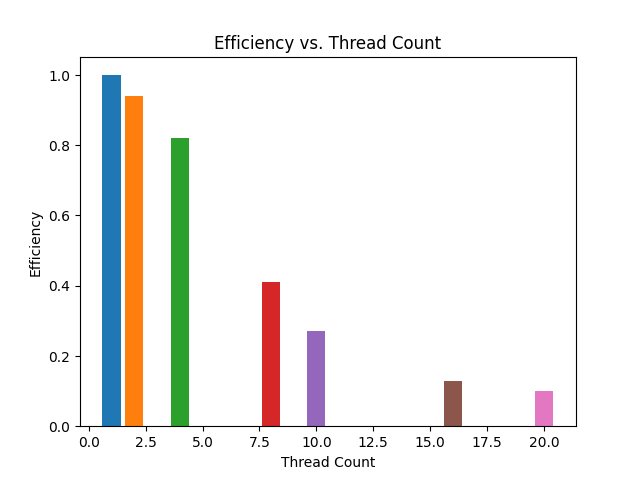
\includegraphics[width=0.8\textwidth]{Figure_2}
		\caption{Efficiency vs. thread count.}
		\label{figure2}
	\end{figure}
	
	\begin{table}
		\centering
		\begin{tabular}{|c|c|c|c|}
			\hline
			\textbf{Thread Count} & \textbf{Execution Time (s)} & \textbf{Speedup} & \textbf{Efficiency} \\
			\hline
			1  & 4616 & 1.00 & 1.00 \\
			2  & 2450 & 1.88 & 0.94 \\
			4  & 1412 & 3.27 & 0.82 \\
			8  & 1397 & 3.30 & 0.41 \\
			10 & 1688 & 2.73 & 0.27 \\
			16 & 2241 & 2.06 & 0.13 \\
			20 & 2381 & 1.94 & 0.10 \\
			\hline
		\end{tabular}
		\caption{Tests showing thread count, execution time in seconds, speedup, and efficiency.}
		\label{table1}
	\end{table}
	
	\clearpage
	
	\section{References}
	\begin{itemize}
		\item \href{https://www.w3schools.com/c/}{https://www.w3schools.com/c/}
		\item \href{https://www.openmp.org/resources/refguides/}{https://www.openmp.org/resources/refguides/}
	\end{itemize}
	
\end{document}